\begin{apendicesenv}
\partapendices
\chapter{Cronograma}
\label{sec:cronograma}
\FloatBarrier
\begin{figure}[!htpd]
		\centering
		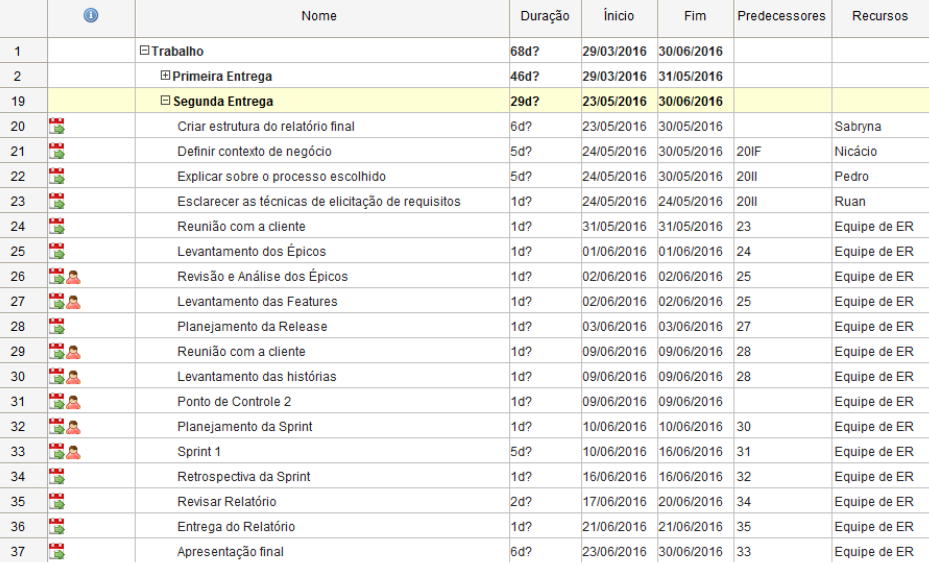
\includegraphics[scale=0.5]{figuras/cronograma}
		\label{img:cronograma}
		\caption{Cronograma de Atividades}
\end{figure}
\chapter{Processo de Engenharia de Requisitos}
\label{sec:processo}
\FloatBarrier
\begin{figure}[!htpd]
		\centering
		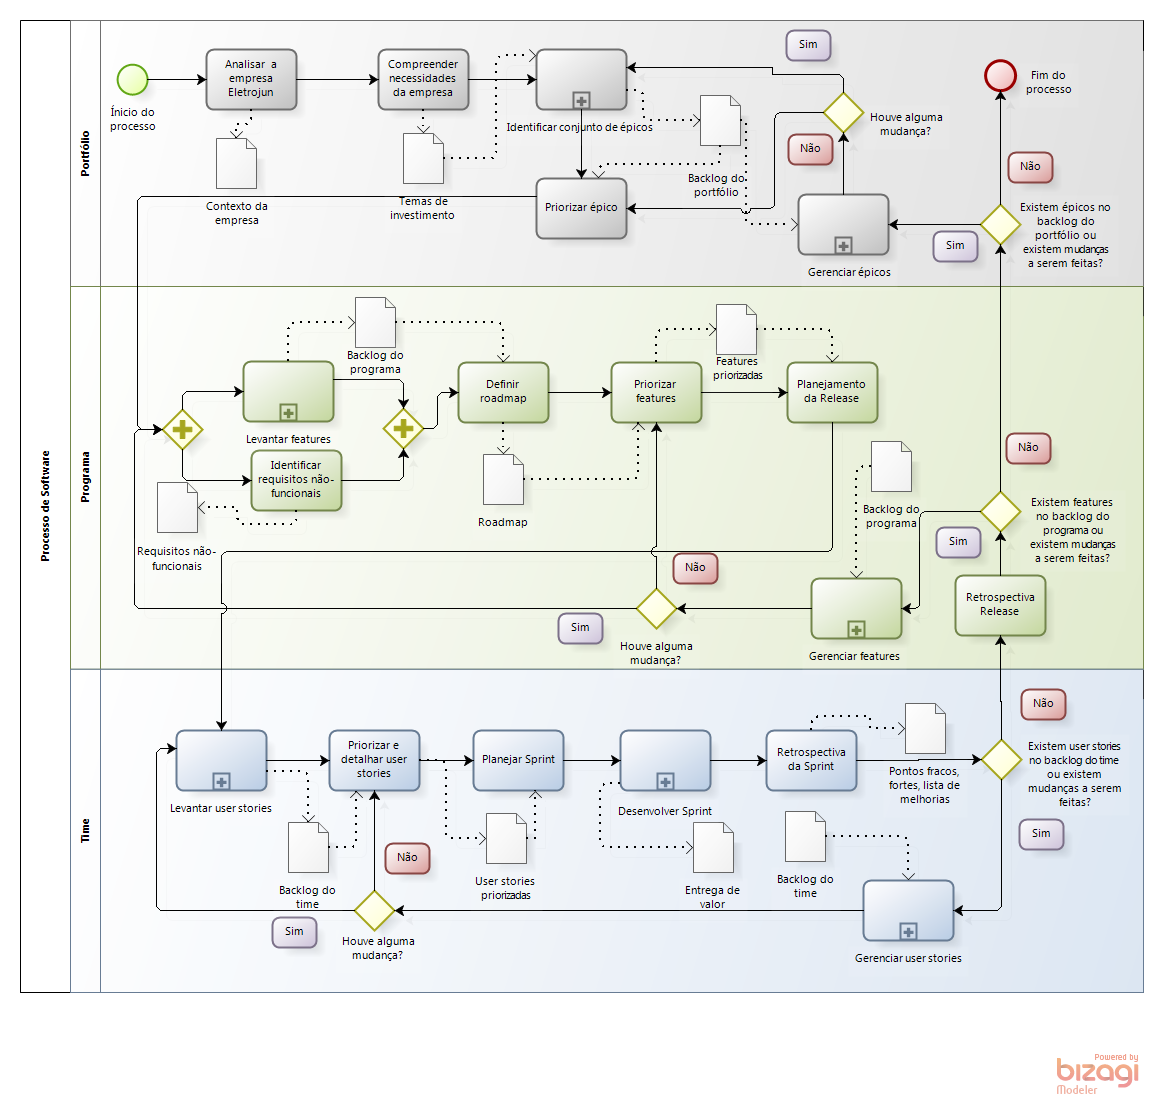
\includegraphics[scale=0.55]{figuras/Eletrojun}
		\label{img:processoeletrojun}
		\caption{Visão geral do processo}
\end{figure}

\chapter{Documento de Visão}
\label{sec:visão}

\textbf{Histórico de Revisões}

\FloatBarrier
\begin{table}[!htpd]
\centering
\caption{My caption}
\label{my-label}
\begin{tabular}{|l|l|l|l|}
\hline
Versão & Data  & Descrição      & Autor(es)                                                                                                \\ \hline
0.5    & 11/06 & Versão Inicial & \begin{tabular}[c]{@{}l@{}}Nicácio Arruda, Pedro Sales, Ruan Herculano,\\  Sabryna de Sousa\end{tabular} \\ \hline
1.0    & 15/06 & Finalização    & \begin{tabular}[c]{@{}l@{}}Nicácio Arruda, Pedro Sales, Ruan Herculano,\\  Sabryna de Sousa\end{tabular} \\ \hline
\end{tabular}
\end{table}

\section{Introdução}

Este documento aborda as características do sistema de Compartilhamento de Projetos, trazendo uma visão do sistema como um tudo, relatando as funcionalidades, o problema que inicial e a solução a ser desenvolvida.

\subsection{Finalidade}

A principal finalidade deste documento é trazer uma visão clara e uma especificação preliminar do software para todos os envolvidos e beneficiários da execução deste.

\subsection{Escopo}

O escopo deste documento visa tornar claro a definição dos requisitos do sistema de compartilhamento de projetos, sendo utilizado a abordagem do SAFe para a elicitação dos mesmos.

\subsection{Visão Geral}

Este documento de visão mostra uma breve introdução sobre o sistema, seguido do posicionamento, onde são abordados os problemas e as motivações para criar este produto. Ele esclarece quem são os envolvidos e  apresenta uma visão geral do produto.

\section{Posicionamento}

\subsection{Oportunidade de Negócios}

A empresa Eletrojun pretende ampliar a sua rede de conexões entre alunos, buscando criar um sistema que auxilie todos da Universidade de Brasília. O principal objetivo deste sistema é a interação entre os usuários do mesmo, a fim de criar uma rede colaborativa em que as pessoas colocam suas ideias, projetos e recebem ajuda de outras pessoas, podendo até mesmo vender suas ideias e inserir um produto no mercado.

\subsection{Descrição do Problema}

\FloatBarrier
\begin{table}[!htpd]
\centering
\caption{My caption}
\label{my-label}
\begin{tabular}{|l|l|}
\hline
O problema de         & Falta de compartilhamento de projetos                                                                                                                                                                                                                                                                                                                                                            \\ \hline
afeta                 & os alunos da Universidade de Brasília                                                                                                                                                                                                                                                                                                                                                            \\ \hline
cujo impacto é        & \begin{tabular}[c]{@{}l@{}}falta de conhecimento por parte dos interessados em colaborar com\\ projetos sobre a existência e o andamento destes, bem como a falta \\ de integração e organização na administração de projetos dos alunos\end{tabular}                                                                                                                                            \\ \hline
uma boa solução seria & \begin{tabular}[c]{@{}l@{}}criar um sistema que pudesse juntar todas as funcionalidades de \\ publicar um projeto, receber ajuda para o desenvolvimento de uma ideia,\\ saber o status de uma atividade, ter uma rede de amigos colaboradores, \\ vender um produto ou uma ideia com ajuda de demais participantes, e ter \\ uma integração dos alunos da Universidade de Brasília.\end{tabular} \\ \hline
\end{tabular}
\end{table}

\subsection{Sentença de Posição do Produto}

\FloatBarrier
\begin{table}[!htpd]
\centering
\caption{My caption}
\label{my-label}
\begin{tabular}{|l|l|}
\hline
Para                                                                                 & os alunos da Universidade de Brasília                                                                                                                                                                                                                                                                                                        \\ \hline
Que                                                                                  & necessitam de uma rede colaborativa                                                                                                                                                                                                                                                                                                          \\ \hline
\begin{tabular}[c]{@{}l@{}}O sistema de compartilhamento \\ de projetos\end{tabular} & é uma rede                                                                                                                                                                                                                                                                                                                                   \\ \hline
Que                                                                                  & \begin{tabular}[c]{@{}l@{}}contém funcionalidades de interação de usuários, administração\\ e compartilhamento de projetos em uma plataforma web\end{tabular}                                                                                                                                                                                \\ \hline
Diferente de                                                                         & Trello, Google Drive, Kickstarter, Instructables                                                                                                                                                                                                                                                                                             \\ \hline
Nosso produto                                                                        & \begin{tabular}[c]{@{}l@{}}tem todas funcionalidades para gestão de um projeto, podendo \\ ser compartilhado com diversos amigos, vendido, ter status\\ sobre o seu progresso e visibilidade, centralizando todas as \\ funcionalidades que necessitariam de diversas plataformas para\\  serem supridas, em uma só plataforma.\end{tabular} \\ \hline
\end{tabular}
\end{table}
\FloatBarrier

\section{Envolvidos e Usuários}

\subsection{Envolvidos}

\FloatBarrier
\begin{table}[!htpd]
\centering
\caption{My caption}
\label{my-label}
\begin{tabular}{|l|l|l|}
\hline
Nome                                                                                 & Descrição                                                                              & Responsabilidades                                                                                                                                              \\ \hline
Mônica                                                                               & \begin{tabular}[c]{@{}l@{}}Diretora da empresa \\ Eletrojun\end{tabular}               & \begin{tabular}[c]{@{}l@{}}Assegurar que os objetivos do software sejam \\ atendidos.\\ Monitorar o projeto\\ Aprovar novas ideias para o sistema\end{tabular} \\ \hline
\begin{tabular}[c]{@{}l@{}}Analistas de Requisitos \\ e Desenvolvedores\end{tabular} & \begin{tabular}[c]{@{}l@{}}Alunos da disciplina\\  Requisitos de Software\end{tabular} & \begin{tabular}[c]{@{}l@{}}Elicitar requisitos \\ Desenvolver parcialmente o sistema\end{tabular}                                                              \\ \hline
\end{tabular}
\end{table}
\FloatBarrier

\subsection{Usuários}

Os usuários da plataforma serão os alunos do Campus Gama da Universidade de Brasília que venham a ter interesse na criação de projetos, visando ter um controle administrativo de colaboradores e tarefas, além de torná-lo visado e comercializável. Também é destinado aos alunos que sejam interessados em contribuir com projetos em andamento.

Os perfis de usuário do sistema são caracterizados por:

\FloatBarrier
\begin{table}[!htpd]
\centering
\caption{My caption}
\label{my-label}
\begin{tabular}{|l|l|}
\hline
Nome                     & Descrição                                                                                                                                    \\ \hline
Usuário do sistema       & \begin{tabular}[c]{@{}l@{}}Usuário que pode criar projetos, tarefas, conversar no chat com \\ seus amigos\end{tabular}                       \\ \hline
Usuário colaborador      & \begin{tabular}[c]{@{}l@{}}Usuário responsável pela execução de tarefas e colaborações com \\ os projetos\end{tabular}                       \\ \hline
Gerente de projeto       & \begin{tabular}[c]{@{}l@{}}Usuário responsável pela administração e distribuição de \\ atividades dos projetos\end{tabular}                  \\ \hline
Administrador do sistema & \begin{tabular}[c]{@{}l@{}}Usuário responsável por manter a plataforma, bem como controle \\ de usuários e projetos cadastrados\end{tabular} \\ \hline
\end{tabular}
\end{table}

\subsubsection{Ambiente dos Usuários}

Todos os usuários da plataforma poderão acessá-la por acesso à internet, via browser de sua preferência por meio do website oficial, utilizando para tal tanto computadores quanto aparelhos mobile.

\section{Visão Geral do Produto}

O sistema consiste num website para auxiliar o desenvolvimento de projetos acadêmicos. Este sistema possibilita que os estudantes compartilhem ideias de projetos e outras informações relevantes sobre o assunto. Os usuários podem contribuir com os projetos existentes de várias formas e podem executar tarefas dentro destes projetos, sendo premiado com moedas do sistema. Os melhores projetos participam de um ranking de projetos onde os usuários podem votar e escolher entre os projetos disponíveis, corroborando para a divulgação do mesmo, de forma a facilitar e propiciar a comercialização. O criador do projeto no sistema pode convidar membros para o projeto e criar atividades. Há também um sistema de chat que possibilita a comunicação entre os usuários.

\end{apendicesenv}
